\documentclass[]{article}
\usepackage{lmodern}
\usepackage{amssymb,amsmath}
\usepackage{ifxetex,ifluatex}
\usepackage{fixltx2e} % provides \textsubscript
\ifnum 0\ifxetex 1\fi\ifluatex 1\fi=0 % if pdftex
  \usepackage[T1]{fontenc}
  \usepackage[utf8]{inputenc}
\else % if luatex or xelatex
  \ifxetex
    \usepackage{mathspec}
  \else
    \usepackage{fontspec}
  \fi
  \defaultfontfeatures{Ligatures=TeX,Scale=MatchLowercase}
\fi
% use upquote if available, for straight quotes in verbatim environments
\IfFileExists{upquote.sty}{\usepackage{upquote}}{}
% use microtype if available
\IfFileExists{microtype.sty}{%
\usepackage[]{microtype}
\UseMicrotypeSet[protrusion]{basicmath} % disable protrusion for tt fonts
}{}
\PassOptionsToPackage{hyphens}{url} % url is loaded by hyperref
\usepackage[unicode=true]{hyperref}
\hypersetup{
            pdftitle={Survivorship},
            pdfauthor={EL Strand},
            pdfborder={0 0 0},
            breaklinks=true}
\urlstyle{same}  % don't use monospace font for urls
\usepackage[margin=1in]{geometry}
\usepackage{color}
\usepackage{fancyvrb}
\newcommand{\VerbBar}{|}
\newcommand{\VERB}{\Verb[commandchars=\\\{\}]}
\DefineVerbatimEnvironment{Highlighting}{Verbatim}{commandchars=\\\{\}}
% Add ',fontsize=\small' for more characters per line
\usepackage{framed}
\definecolor{shadecolor}{RGB}{248,248,248}
\newenvironment{Shaded}{\begin{snugshade}}{\end{snugshade}}
\newcommand{\KeywordTok}[1]{\textcolor[rgb]{0.13,0.29,0.53}{\textbf{#1}}}
\newcommand{\DataTypeTok}[1]{\textcolor[rgb]{0.13,0.29,0.53}{#1}}
\newcommand{\DecValTok}[1]{\textcolor[rgb]{0.00,0.00,0.81}{#1}}
\newcommand{\BaseNTok}[1]{\textcolor[rgb]{0.00,0.00,0.81}{#1}}
\newcommand{\FloatTok}[1]{\textcolor[rgb]{0.00,0.00,0.81}{#1}}
\newcommand{\ConstantTok}[1]{\textcolor[rgb]{0.00,0.00,0.00}{#1}}
\newcommand{\CharTok}[1]{\textcolor[rgb]{0.31,0.60,0.02}{#1}}
\newcommand{\SpecialCharTok}[1]{\textcolor[rgb]{0.00,0.00,0.00}{#1}}
\newcommand{\StringTok}[1]{\textcolor[rgb]{0.31,0.60,0.02}{#1}}
\newcommand{\VerbatimStringTok}[1]{\textcolor[rgb]{0.31,0.60,0.02}{#1}}
\newcommand{\SpecialStringTok}[1]{\textcolor[rgb]{0.31,0.60,0.02}{#1}}
\newcommand{\ImportTok}[1]{#1}
\newcommand{\CommentTok}[1]{\textcolor[rgb]{0.56,0.35,0.01}{\textit{#1}}}
\newcommand{\DocumentationTok}[1]{\textcolor[rgb]{0.56,0.35,0.01}{\textbf{\textit{#1}}}}
\newcommand{\AnnotationTok}[1]{\textcolor[rgb]{0.56,0.35,0.01}{\textbf{\textit{#1}}}}
\newcommand{\CommentVarTok}[1]{\textcolor[rgb]{0.56,0.35,0.01}{\textbf{\textit{#1}}}}
\newcommand{\OtherTok}[1]{\textcolor[rgb]{0.56,0.35,0.01}{#1}}
\newcommand{\FunctionTok}[1]{\textcolor[rgb]{0.00,0.00,0.00}{#1}}
\newcommand{\VariableTok}[1]{\textcolor[rgb]{0.00,0.00,0.00}{#1}}
\newcommand{\ControlFlowTok}[1]{\textcolor[rgb]{0.13,0.29,0.53}{\textbf{#1}}}
\newcommand{\OperatorTok}[1]{\textcolor[rgb]{0.81,0.36,0.00}{\textbf{#1}}}
\newcommand{\BuiltInTok}[1]{#1}
\newcommand{\ExtensionTok}[1]{#1}
\newcommand{\PreprocessorTok}[1]{\textcolor[rgb]{0.56,0.35,0.01}{\textit{#1}}}
\newcommand{\AttributeTok}[1]{\textcolor[rgb]{0.77,0.63,0.00}{#1}}
\newcommand{\RegionMarkerTok}[1]{#1}
\newcommand{\InformationTok}[1]{\textcolor[rgb]{0.56,0.35,0.01}{\textbf{\textit{#1}}}}
\newcommand{\WarningTok}[1]{\textcolor[rgb]{0.56,0.35,0.01}{\textbf{\textit{#1}}}}
\newcommand{\AlertTok}[1]{\textcolor[rgb]{0.94,0.16,0.16}{#1}}
\newcommand{\ErrorTok}[1]{\textcolor[rgb]{0.64,0.00,0.00}{\textbf{#1}}}
\newcommand{\NormalTok}[1]{#1}
\usepackage{graphicx,grffile}
\makeatletter
\def\maxwidth{\ifdim\Gin@nat@width>\linewidth\linewidth\else\Gin@nat@width\fi}
\def\maxheight{\ifdim\Gin@nat@height>\textheight\textheight\else\Gin@nat@height\fi}
\makeatother
% Scale images if necessary, so that they will not overflow the page
% margins by default, and it is still possible to overwrite the defaults
% using explicit options in \includegraphics[width, height, ...]{}
\setkeys{Gin}{width=\maxwidth,height=\maxheight,keepaspectratio}
\IfFileExists{parskip.sty}{%
\usepackage{parskip}
}{% else
\setlength{\parindent}{0pt}
\setlength{\parskip}{6pt plus 2pt minus 1pt}
}
\setlength{\emergencystretch}{3em}  % prevent overfull lines
\providecommand{\tightlist}{%
  \setlength{\itemsep}{0pt}\setlength{\parskip}{0pt}}
\setcounter{secnumdepth}{0}
% Redefines (sub)paragraphs to behave more like sections
\ifx\paragraph\undefined\else
\let\oldparagraph\paragraph
\renewcommand{\paragraph}[1]{\oldparagraph{#1}\mbox{}}
\fi
\ifx\subparagraph\undefined\else
\let\oldsubparagraph\subparagraph
\renewcommand{\subparagraph}[1]{\oldsubparagraph{#1}\mbox{}}
\fi

% set default figure placement to htbp
\makeatletter
\def\fps@figure{htbp}
\makeatother


\title{Survivorship}
\author{EL Strand}
\date{6/10/2020}

\begin{document}
\maketitle

Clear workspace.

\begin{Shaded}
\begin{Highlighting}[]
\KeywordTok{rm}\NormalTok{(}\DataTypeTok{list=}\KeywordTok{ls}\NormalTok{())}
\end{Highlighting}
\end{Shaded}

Installing and loading required libraries.

\begin{Shaded}
\begin{Highlighting}[]
\ControlFlowTok{if}\NormalTok{ (}\StringTok{"tidyr"} \OperatorTok\StringTok{ }\KeywordTok{rownames}\NormalTok{(}\KeywordTok{installed.packages}\NormalTok{()) }\OperatorTok{==}\StringTok{ 'FALSE'}\NormalTok{) }\KeywordTok{install.packages}\NormalTok{(}\StringTok{'tidyr'}\NormalTok{) }
\ControlFlowTok{if}\NormalTok{ (}\StringTok{"tidyverse"} \OperatorTok\StringTok{ }\KeywordTok{rownames}\NormalTok{(}\KeywordTok{installed.packages}\NormalTok{()) }\OperatorTok{==}\StringTok{ 'FALSE'}\NormalTok{) }\KeywordTok{install.packages}\NormalTok{(}\StringTok{'tidyverse'}\NormalTok{) }
\ControlFlowTok{if}\NormalTok{ (}\StringTok{"reshape"} \OperatorTok\StringTok{ }\KeywordTok{rownames}\NormalTok{(}\KeywordTok{installed.packages}\NormalTok{()) }\OperatorTok{==}\StringTok{ 'FALSE'}\NormalTok{) }\KeywordTok{install.packages}\NormalTok{(}\StringTok{'reshape'}\NormalTok{) }
\ControlFlowTok{if}\NormalTok{ (}\StringTok{"stringr"} \OperatorTok\StringTok{ }\KeywordTok{rownames}\NormalTok{(}\KeywordTok{installed.packages}\NormalTok{()) }\OperatorTok{==}\StringTok{ 'FALSE'}\NormalTok{) }\KeywordTok{install.packages}\NormalTok{(}\StringTok{'stringr'}\NormalTok{) }
\ControlFlowTok{if}\NormalTok{ (}\StringTok{"survival"} \OperatorTok\StringTok{ }\KeywordTok{rownames}\NormalTok{(}\KeywordTok{installed.packages}\NormalTok{()) }\OperatorTok{==}\StringTok{ 'FALSE'}\NormalTok{) }\KeywordTok{install.packages}\NormalTok{(}\StringTok{'survival'}\NormalTok{) }
\ControlFlowTok{if}\NormalTok{ (}\StringTok{"ranger"} \OperatorTok\StringTok{ }\KeywordTok{rownames}\NormalTok{(}\KeywordTok{installed.packages}\NormalTok{()) }\OperatorTok{==}\StringTok{ 'FALSE'}\NormalTok{) }\KeywordTok{install.packages}\NormalTok{(}\StringTok{'ranger'}\NormalTok{) }
\ControlFlowTok{if}\NormalTok{ (}\StringTok{"ggplot2"} \OperatorTok\StringTok{ }\KeywordTok{rownames}\NormalTok{(}\KeywordTok{installed.packages}\NormalTok{()) }\OperatorTok{==}\StringTok{ 'FALSE'}\NormalTok{) }\KeywordTok{install.packages}\NormalTok{(}\StringTok{'ggplot2'}\NormalTok{) }
\ControlFlowTok{if}\NormalTok{ (}\StringTok{"dplyr"} \OperatorTok\StringTok{ }\KeywordTok{rownames}\NormalTok{(}\KeywordTok{installed.packages}\NormalTok{()) }\OperatorTok{==}\StringTok{ 'FALSE'}\NormalTok{) }\KeywordTok{install.packages}\NormalTok{(}\StringTok{'dplyr'}\NormalTok{) }
\ControlFlowTok{if}\NormalTok{ (}\StringTok{"ggfortify"} \OperatorTok\StringTok{ }\KeywordTok{rownames}\NormalTok{(}\KeywordTok{installed.packages}\NormalTok{()) }\OperatorTok{==}\StringTok{ 'FALSE'}\NormalTok{) }\KeywordTok{install.packages}\NormalTok{(}\StringTok{'ggfortify'}\NormalTok{) }
\ControlFlowTok{if}\NormalTok{ (}\StringTok{"gridExtra"} \OperatorTok\StringTok{ }\KeywordTok{rownames}\NormalTok{(}\KeywordTok{installed.packages}\NormalTok{()) }\OperatorTok{==}\StringTok{ 'FALSE'}\NormalTok{) }\KeywordTok{install.packages}\NormalTok{(}\StringTok{'gridExtra'}\NormalTok{) }
\ControlFlowTok{if}\NormalTok{ (}\StringTok{"survminer"} \OperatorTok\StringTok{ }\KeywordTok{rownames}\NormalTok{(}\KeywordTok{installed.packages}\NormalTok{()) }\OperatorTok{==}\StringTok{ 'FALSE'}\NormalTok{) }\KeywordTok{install.packages}\NormalTok{(}\StringTok{'survminer'}\NormalTok{) }

\CommentTok{#Read in required libraries}
\NormalTok{##### Include Versions of libraries}
\KeywordTok{library}\NormalTok{(tidyr)}
\KeywordTok{library}\NormalTok{(tidyverse)}
\end{Highlighting}
\end{Shaded}

\begin{verbatim}
## -- Attaching packages --------------------------------------- tidyverse 1.3.0 --
\end{verbatim}

\begin{verbatim}
## v ggplot2 3.3.1     v dplyr   0.8.5
## v tibble  2.1.3     v stringr 1.4.0
## v readr   1.3.1     v forcats 0.5.0
## v purrr   0.3.3
\end{verbatim}

\begin{verbatim}
## -- Conflicts ------------------------------------------ tidyverse_conflicts() --
## x dplyr::filter() masks stats::filter()
## x dplyr::lag()    masks stats::lag()
\end{verbatim}

\begin{Shaded}
\begin{Highlighting}[]
\KeywordTok{library}\NormalTok{(reshape)}
\end{Highlighting}
\end{Shaded}

\begin{verbatim}
## 
## Attaching package: 'reshape'
\end{verbatim}

\begin{verbatim}
## The following object is masked from 'package:dplyr':
## 
##     rename
\end{verbatim}

\begin{verbatim}
## The following objects are masked from 'package:tidyr':
## 
##     expand, smiths
\end{verbatim}

\begin{Shaded}
\begin{Highlighting}[]
\KeywordTok{library}\NormalTok{(stringr)}
\KeywordTok{library}\NormalTok{(survival)}
\KeywordTok{library}\NormalTok{(ranger)}
\KeywordTok{library}\NormalTok{(ggplot2)}
\KeywordTok{library}\NormalTok{(dplyr)}
\KeywordTok{library}\NormalTok{(ggfortify)}
\KeywordTok{library}\NormalTok{(gridExtra)}
\end{Highlighting}
\end{Shaded}

\begin{verbatim}
## 
## Attaching package: 'gridExtra'
\end{verbatim}

\begin{verbatim}
## The following object is masked from 'package:dplyr':
## 
##     combine
\end{verbatim}

\begin{Shaded}
\begin{Highlighting}[]
\KeywordTok{library}\NormalTok{(survminer)}
\end{Highlighting}
\end{Shaded}

\begin{verbatim}
## Loading required package: ggpubr
\end{verbatim}

\begin{verbatim}
## Loading required package: magrittr
\end{verbatim}

\begin{verbatim}
## 
## Attaching package: 'magrittr'
\end{verbatim}

\begin{verbatim}
## The following object is masked from 'package:purrr':
## 
##     set_names
\end{verbatim}

\begin{verbatim}
## The following object is masked from 'package:tidyr':
## 
##     extract
\end{verbatim}

Loading dataframes.

\begin{Shaded}
\begin{Highlighting}[]
\NormalTok{Data <-}\StringTok{ }\KeywordTok{read.csv}\NormalTok{(}\StringTok{"Physiology_variables/coral_survivorship_QC.csv"}\NormalTok{, }\DataTypeTok{header=}\NormalTok{T, }\DataTypeTok{sep=}\StringTok{","}\NormalTok{, }\DataTypeTok{na.string=}\StringTok{"NA"}\NormalTok{, }\DataTypeTok{stringsAsFactors =}\NormalTok{ F) }\CommentTok{#read in data file}
\NormalTok{Tank.Info <-}\StringTok{ }\KeywordTok{read.csv}\NormalTok{(}\StringTok{"Environmental_data/Tank_to_Treatment.csv"}\NormalTok{, }\DataTypeTok{header=}\NormalTok{T, }\DataTypeTok{sep=}\StringTok{","}\NormalTok{, }\DataTypeTok{na.string=}\StringTok{"NA"}\NormalTok{) }\CommentTok{#read in data file }
\NormalTok{Data.Trt <-}\StringTok{ }\KeywordTok{merge}\NormalTok{(Data, Tank.Info, }\DataTypeTok{by=}\StringTok{"Tank"}\NormalTok{)}
\end{Highlighting}
\end{Shaded}

Replace sampled with alive.

\begin{Shaded}
\begin{Highlighting}[]
\NormalTok{Data.Trt.x <-}\StringTok{ }\NormalTok{Data.Trt }\OperatorTok\StringTok{ }\KeywordTok{mutate_if}\NormalTok{(is.character, str_replace_all, }\DataTypeTok{pattern =} \StringTok{'sampled'}\NormalTok{, }\DataTypeTok{replacement =} \StringTok{'alive'}\NormalTok{)}
\NormalTok{Data.Trt.x}\OperatorTok{$}\NormalTok{lifespan <-}\StringTok{ }\KeywordTok{rowSums}\NormalTok{(Data.Trt.x[,}\DecValTok{10}\OperatorTok{:}\DecValTok{120}\NormalTok{] }\OperatorTok{==}\StringTok{ "alive"}\NormalTok{)}
\NormalTok{Data.Trt.x}\OperatorTok{$}\NormalTok{status <-}\StringTok{ }\KeywordTok{as.numeric}\NormalTok{(}\KeywordTok{as.factor}\NormalTok{(Data.Trt.x}\OperatorTok{$}\NormalTok{Day.}\DecValTok{110}\NormalTok{))}
\end{Highlighting}
\end{Shaded}

Survivorship analysis.

\begin{Shaded}
\begin{Highlighting}[]
\NormalTok{### Montipora capitata}
\NormalTok{Mc.Data <-}\StringTok{ }\KeywordTok{subset}\NormalTok{(Data.Trt.x, Species}\OperatorTok{==}\StringTok{"Mcapitata"}\NormalTok{)}
\NormalTok{Mc.Data}\OperatorTok{$}\NormalTok{group <-}\StringTok{ }\KeywordTok{paste0}\NormalTok{(Mc.Data}\OperatorTok{$}\NormalTok{Treatment) }
\NormalTok{Mc.km <-}\StringTok{ }\KeywordTok{with}\NormalTok{(Mc.Data, }\KeywordTok{Surv}\NormalTok{(lifespan, status))}
\NormalTok{Mc.km_fit <-}\StringTok{ }\KeywordTok{survfit}\NormalTok{(}\KeywordTok{Surv}\NormalTok{(lifespan, status) }\OperatorTok{~}\StringTok{ }\NormalTok{Treatment, }\DataTypeTok{data=}\NormalTok{Mc.Data)}
\KeywordTok{summary}\NormalTok{(Mc.km_fit)}
\end{Highlighting}
\end{Shaded}

\begin{verbatim}
## Call: survfit(formula = Surv(lifespan, status) ~ Treatment, data = Mc.Data)
## 
## 354 observations deleted due to missingness 
##                 Treatment=ATAC 
##  time n.risk n.event survival std.err lower 95% CI upper 95% CI
##    46     22       1    0.955  0.0444        0.871            1
##    55     21       1    0.909  0.0613        0.797            1
## 
##                 Treatment=ATHC 
##  time n.risk n.event survival std.err lower 95% CI upper 95% CI
##    12     26       1    0.962  0.0377        0.890            1
##    30     25       1    0.923  0.0523        0.826            1
##   108     24       1    0.885  0.0627        0.770            1
## 
##                 Treatment=HTAC 
##  time n.risk n.event survival std.err lower 95% CI upper 95% CI
##    38     18       2    0.889  0.0741        0.755            1
##    81     16       1    0.833  0.0878        0.678            1
## 
##                 Treatment=HTHC 
##  time n.risk n.event survival std.err lower 95% CI upper 95% CI
##    30     22       1    0.955  0.0444        0.871        1.000
##    47     21       1    0.909  0.0613        0.797        1.000
##    49     20       2    0.818  0.0822        0.672        0.996
##    54     18       1    0.773  0.0893        0.616        0.969
##    55     17       1    0.727  0.0950        0.563        0.939
##    97     16       1    0.682  0.0993        0.513        0.907
\end{verbatim}

\begin{Shaded}
\begin{Highlighting}[]
\NormalTok{cols <-}\StringTok{ }\KeywordTok{c}\NormalTok{(}\StringTok{"lightblue"}\NormalTok{, }\StringTok{"blue"}\NormalTok{, }\StringTok{"salmon"}\NormalTok{, }\StringTok{"red3"}\NormalTok{)}
\NormalTok{MC.sur <-}\StringTok{ }\KeywordTok{summary}\NormalTok{(Mc.km_fit, }\DataTypeTok{times =} \KeywordTok{c}\NormalTok{(}\DecValTok{1}\OperatorTok{:}\DecValTok{58}\NormalTok{))}
\NormalTok{Mc.km_fit <-}\StringTok{ }\KeywordTok{survfit}\NormalTok{(}\KeywordTok{Surv}\NormalTok{(lifespan, status) }\OperatorTok{~}\StringTok{ }\NormalTok{Treatment, }\DataTypeTok{data=}\NormalTok{Mc.Data)}
\KeywordTok{autoplot}\NormalTok{(Mc.km_fit)}
\end{Highlighting}
\end{Shaded}

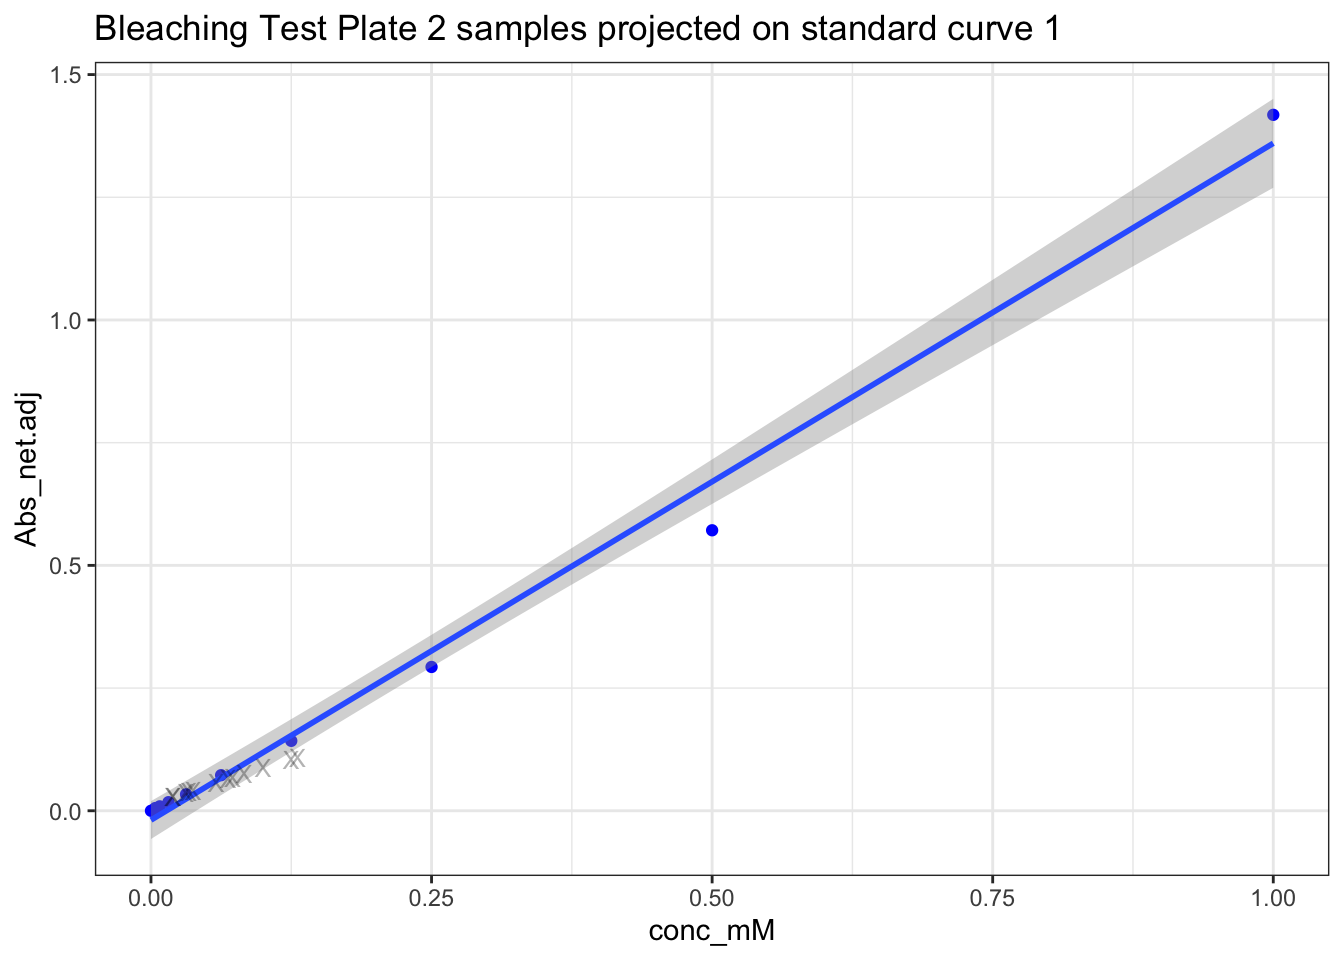
\includegraphics{Survivorship_files/figure-latex/unnamed-chunk-5-1.pdf}

\begin{Shaded}
\begin{Highlighting}[]
\NormalTok{### Pocillopora acuta}
\NormalTok{Pa.Data <-}\StringTok{ }\KeywordTok{subset}\NormalTok{(Data.Trt.x, Species}\OperatorTok{==}\StringTok{"Pacuta"}\NormalTok{)}
\NormalTok{Pa.km <-}\StringTok{ }\KeywordTok{with}\NormalTok{(Pa.Data, }\KeywordTok{Surv}\NormalTok{(lifespan, status))}
\NormalTok{Pa.km_fit <-}\StringTok{ }\KeywordTok{survfit}\NormalTok{(}\KeywordTok{Surv}\NormalTok{(lifespan, status) }\OperatorTok{~}\StringTok{ }\NormalTok{Treatment, }\DataTypeTok{data=}\NormalTok{Pa.Data) }\CommentTok{#*Origin}
\NormalTok{Pa.sur <-}\StringTok{ }\KeywordTok{summary}\NormalTok{(Pa.km_fit, }\DataTypeTok{times =} \KeywordTok{c}\NormalTok{(}\DecValTok{1}\OperatorTok{:}\DecValTok{58}\NormalTok{))}
\KeywordTok{autoplot}\NormalTok{(Pa.km_fit)}
\end{Highlighting}
\end{Shaded}

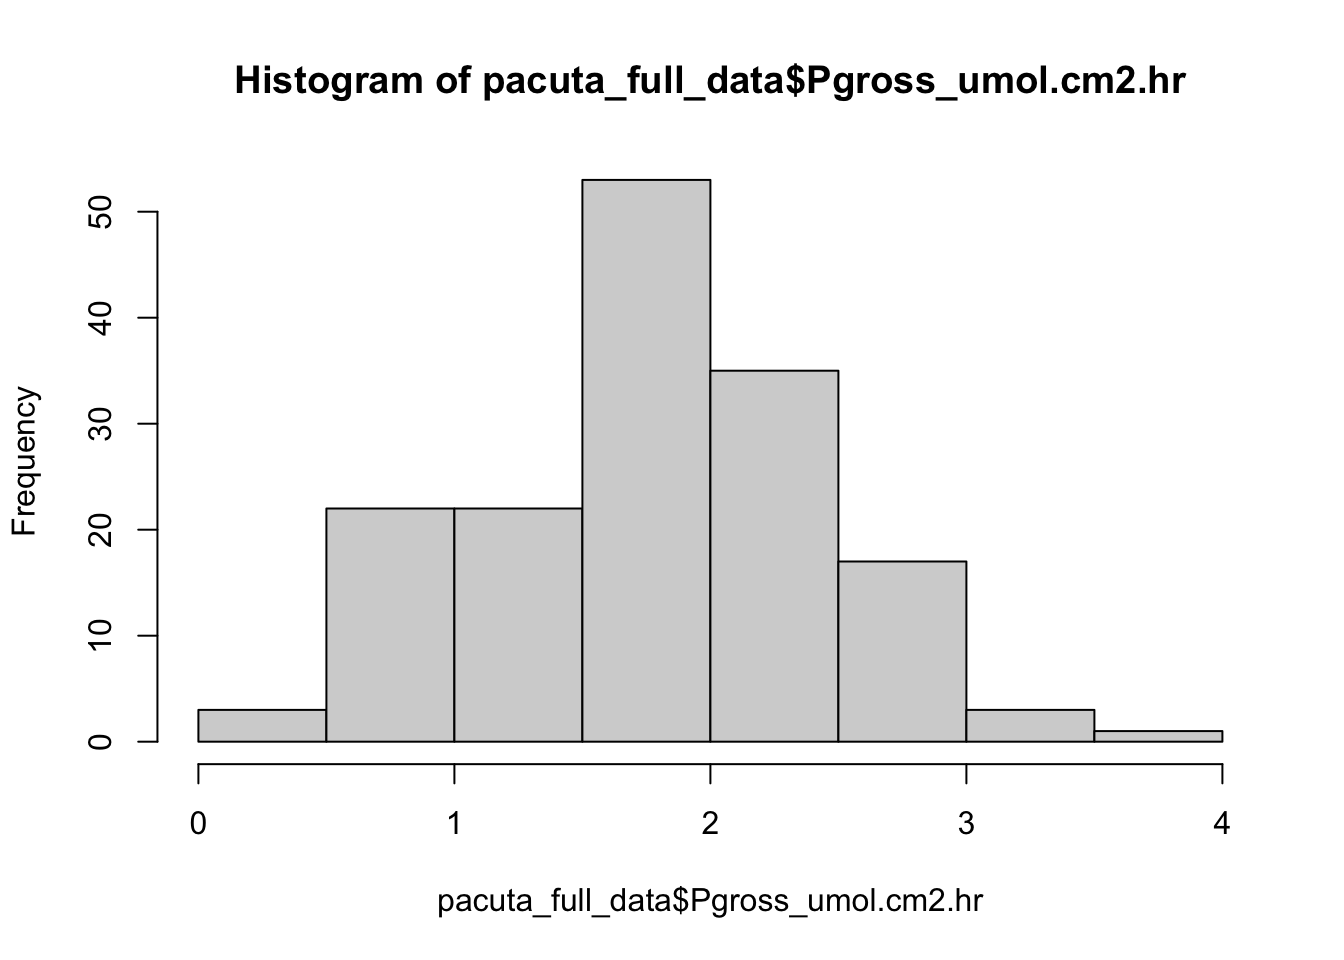
\includegraphics{Survivorship_files/figure-latex/unnamed-chunk-5-2.pdf}

Plotting survivorship analysis.

\begin{Shaded}
\begin{Highlighting}[]
\NormalTok{## Montipora capitata}
\NormalTok{Fig.Mcap <-}\StringTok{ }\KeywordTok{ggsurvplot}\NormalTok{(Mc.km_fit, }\DataTypeTok{data=}\NormalTok{Mc.Data, }\DataTypeTok{size =} \DecValTok{1}\NormalTok{,  }\CommentTok{# change line size}
           \DataTypeTok{linetype =} \StringTok{"strata"}\NormalTok{, }\CommentTok{# change line type by groups}
           \DataTypeTok{break.time.by =} \DecValTok{7}\NormalTok{, }\CommentTok{# break time axis}
           \DataTypeTok{palette =} \KeywordTok{c}\NormalTok{(}\StringTok{"blue"}\NormalTok{, }\StringTok{"lightblue"}\NormalTok{, }\StringTok{"salmon"}\NormalTok{, }\StringTok{"red3"}\NormalTok{), }\CommentTok{# custom color palette}
           \DataTypeTok{conf.int =} \OtherTok{TRUE}\NormalTok{, }\CommentTok{# Add confidence interval}
           \DataTypeTok{legend.title =} \StringTok{""}\NormalTok{, }\CommentTok{# remove legend title}
           \DataTypeTok{title =} \StringTok{"Montipora capitata"}\NormalTok{,}
           \DataTypeTok{xlab =} \StringTok{"Time in days"}\NormalTok{,}
           \DataTypeTok{font.title =} \KeywordTok{c}\NormalTok{(}\DecValTok{14}\NormalTok{, }\StringTok{"bold.italic"}\NormalTok{, }\StringTok{"black"}\NormalTok{), }\CommentTok{#title italicized}
           \DataTypeTok{legend.labs =} \KeywordTok{c}\NormalTok{(}\StringTok{"ATAC"}\NormalTok{, }\StringTok{"ATHC"}\NormalTok{,}\StringTok{"HTAC"}\NormalTok{, }\StringTok{"HTHC"}\NormalTok{), }\DataTypeTok{pval =} \OtherTok{TRUE}\NormalTok{, }\CommentTok{# Add p-value and change legend labels}
           \DataTypeTok{legend=}\KeywordTok{c}\NormalTok{(}\FloatTok{0.115}\NormalTok{, }\FloatTok{0.45}\NormalTok{))}
\NormalTok{Fig.Mcap}
\end{Highlighting}
\end{Shaded}

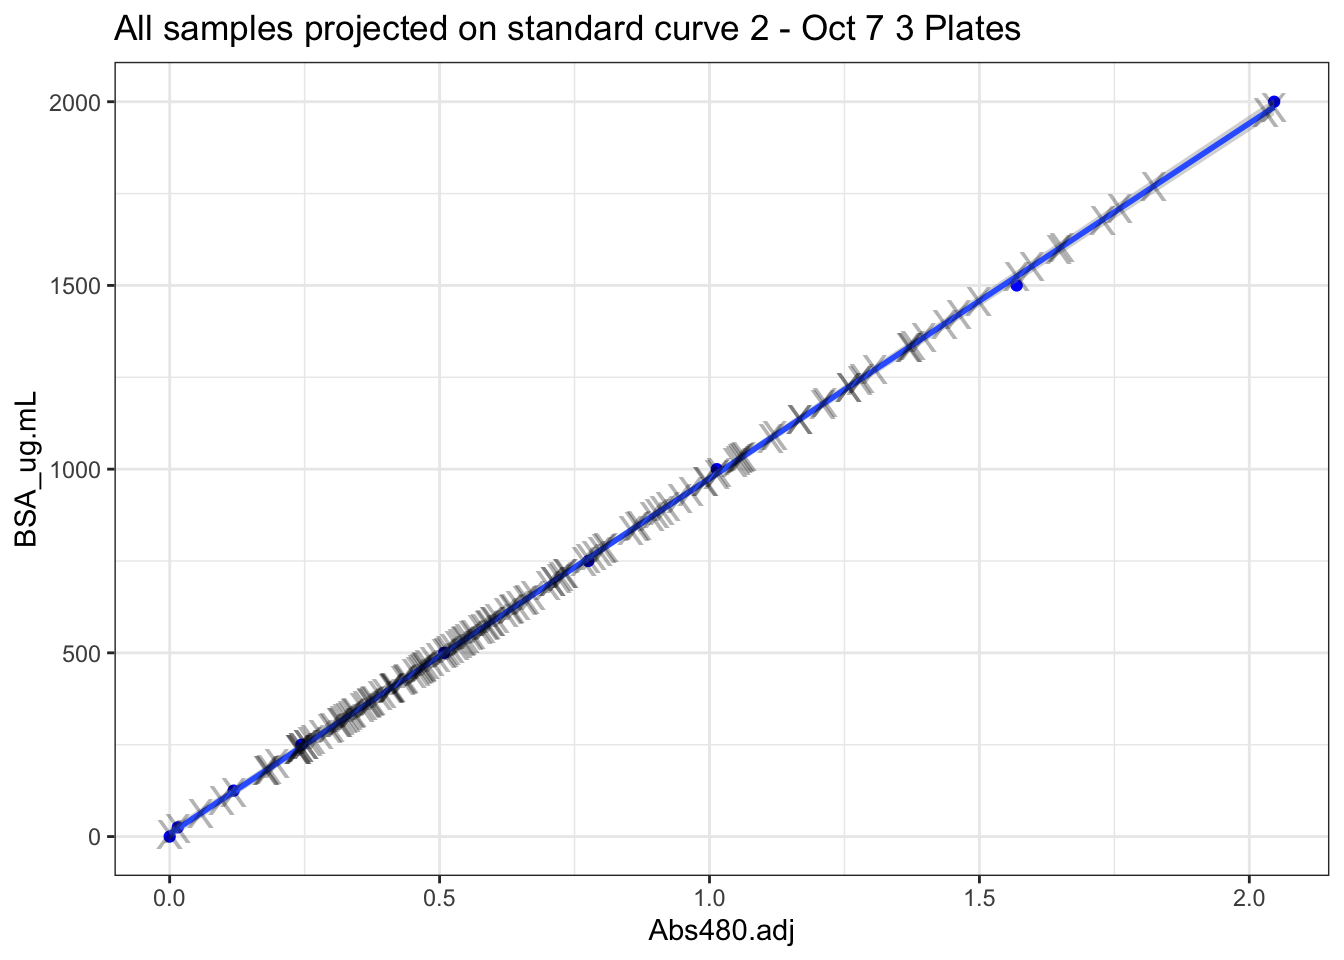
\includegraphics{Survivorship_files/figure-latex/unnamed-chunk-6-1.pdf}

\begin{Shaded}
\begin{Highlighting}[]
\NormalTok{## Pocillopora acuta}
\NormalTok{Fig.PA <-}\StringTok{ }\KeywordTok{ggsurvplot}\NormalTok{(Pa.km_fit, }\DataTypeTok{data=}\NormalTok{Pa.Data, }\DataTypeTok{size =} \DecValTok{1}\NormalTok{,  }\CommentTok{# change line size}
           \DataTypeTok{linetype =} \StringTok{"strata"}\NormalTok{, }\CommentTok{# change line type by groups}
           \DataTypeTok{break.time.by =} \DecValTok{7}\NormalTok{, }\CommentTok{# break time axis}
           \DataTypeTok{palette =} \KeywordTok{c}\NormalTok{(}\StringTok{"blue"}\NormalTok{, }\StringTok{"lightblue"}\NormalTok{, }\StringTok{"salmon"}\NormalTok{, }\StringTok{"red3"}\NormalTok{), }\CommentTok{# custom color palette}
           \DataTypeTok{conf.int =} \OtherTok{TRUE}\NormalTok{, }\CommentTok{# Add confidence interval}
           \DataTypeTok{legend.title =} \StringTok{""}\NormalTok{, }\CommentTok{# remove legend title}
           \DataTypeTok{title =} \StringTok{"Pocillopora acuta"}\NormalTok{,}
           \DataTypeTok{xlab =} \StringTok{"Time in days"}\NormalTok{,}
           \DataTypeTok{font.title =} \KeywordTok{c}\NormalTok{(}\DecValTok{14}\NormalTok{, }\StringTok{"bold.italic"}\NormalTok{, }\StringTok{"black"}\NormalTok{), }\CommentTok{#title italicized}
           \DataTypeTok{legend.labs =} \KeywordTok{c}\NormalTok{(}\StringTok{"ATAC"}\NormalTok{, }\StringTok{"ATHC"}\NormalTok{,}\StringTok{"HTAC"}\NormalTok{, }\StringTok{"HTHC"}\NormalTok{), }\DataTypeTok{pval =} \OtherTok{TRUE}\NormalTok{, }\CommentTok{# Add p-value and change legend labels}
           \DataTypeTok{legend=}\KeywordTok{c}\NormalTok{(}\FloatTok{0.115}\NormalTok{, }\FloatTok{0.45}\NormalTok{))}
\NormalTok{Fig.PA}
\end{Highlighting}
\end{Shaded}

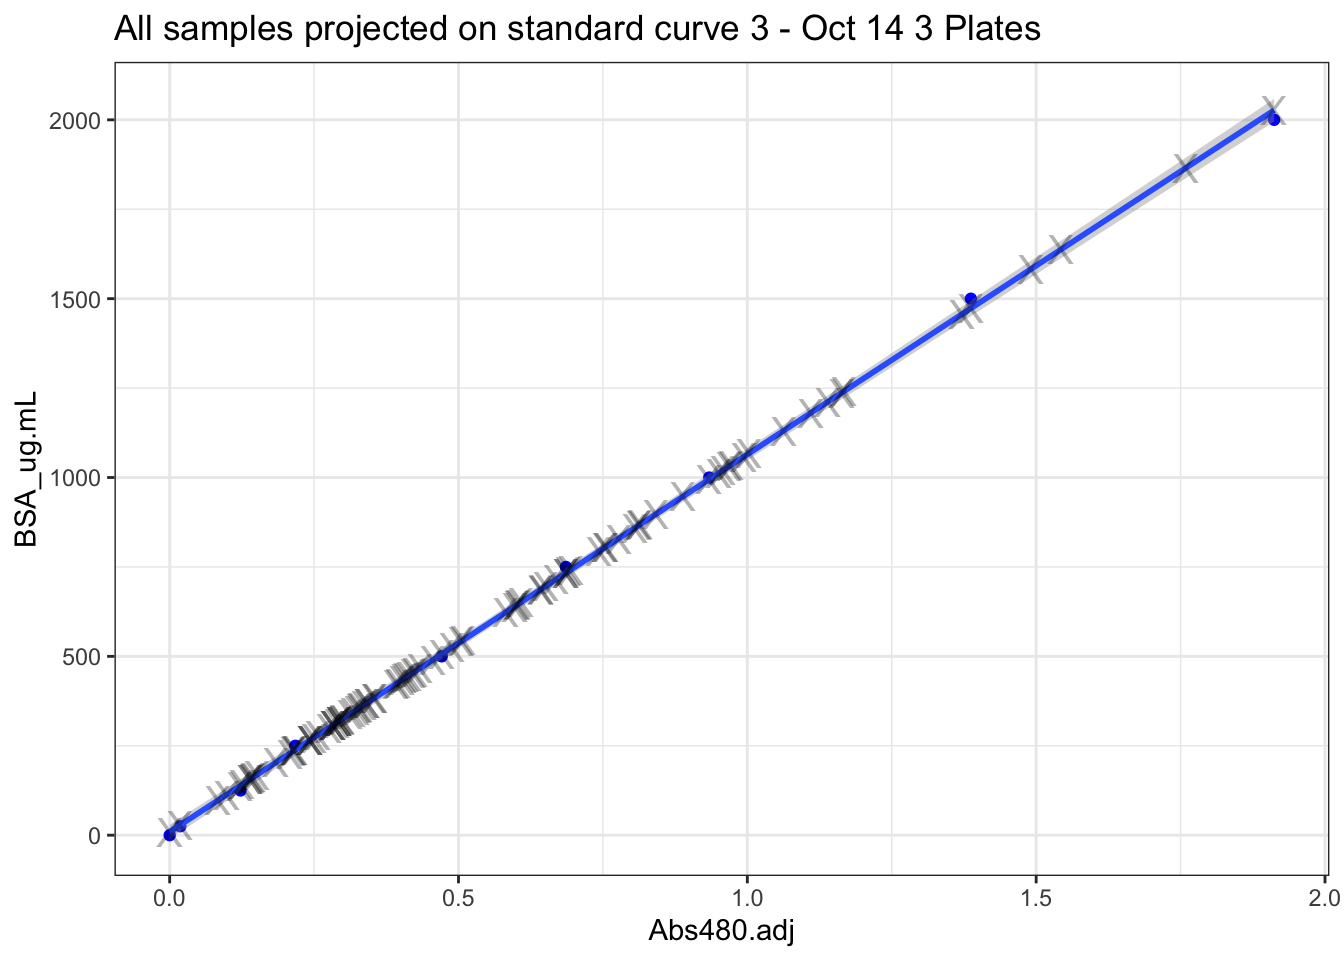
\includegraphics{Survivorship_files/figure-latex/unnamed-chunk-6-2.pdf}

\begin{Shaded}
\begin{Highlighting}[]
\CommentTok{# Surv.figs <- arrange_ggsurvplots(Fig.Mcap, Fig.PA, print = FALSE)}
  \CommentTok{# ncol = 1,}
  \CommentTok{# nrow = 2,}
  \CommentTok{# title = "Survivorship Probability")}

\CommentTok{# ggsave(Fig.PA, file = "Physiology_variables/Poc_Survival.pdf", print(Fig.PA))}

\KeywordTok{png}\NormalTok{(}\StringTok{"Physiology_variables/Poc_Survival.png"}\NormalTok{)}
\KeywordTok{print}\NormalTok{(Fig.PA, }\DataTypeTok{newpage =} \OtherTok{FALSE}\NormalTok{)}
\KeywordTok{dev.off}\NormalTok{()}
\end{Highlighting}
\end{Shaded}

\begin{verbatim}
## pdf 
##   2
\end{verbatim}

\begin{Shaded}
\begin{Highlighting}[]
\KeywordTok{jpeg}\NormalTok{(}\StringTok{"Physiology_variables/Mont_Survival.jpeg"}\NormalTok{)}
\KeywordTok{print}\NormalTok{(Fig.Mcap, }\DataTypeTok{newpage =} \OtherTok{FALSE}\NormalTok{)}
\KeywordTok{dev.off}\NormalTok{()}
\end{Highlighting}
\end{Shaded}

\begin{verbatim}
## pdf 
##   2
\end{verbatim}

\begin{Shaded}
\begin{Highlighting}[]
\CommentTok{# ggsave(Fig.PA, file = "Physiology_variables/Poc_Survival.pdf", width = 8, height = 11)}
\CommentTok{# ggsave(Fig.Mcap, file = "Physiology_variables/Mont_Survival.pdf", width = 8, height = 11)}
\end{Highlighting}
\end{Shaded}

\end{document}
